% =====================================================================
% Paper section: meme-level RALE alignment in SMACv2.
% Drop into the existing alignment section (e.g. \S5.4 in the paper).
% Requires: \usepackage{booktabs, graphicx, amsmath, amssymb, multirow}.
% =====================================================================

\subsection{Meme-Level Replication--Reward Alignment in SMACv2}
\label{sec:rale-smacv2}

\paragraph{Method.}
We measure the meme-level alignment between host fitness $F$ and replicative
fitness $R$ \emph{after} phase-2 adaptation, treating each agent--step as a
host that carries a latent meme $z\in\mathbb{R}^{d_z}$ produced by the
adapter's persistent state cell. For each method
$m\in\{\textsc{ALEC},\,\textsc{MAPPO}\}$ and each seed $\sigma$ we roll out
$25$ deterministic-action evaluation episodes and log the tuple
$(z_t,\,z_{t+1},\,r_t,\,G_e,\,\mathbf{1}[\text{done}])$ for every agent at
every step. Both adapters are initialised with a small symmetry-breaking
Gaussian perturbation ($\sigma\!=\!0.05$) on the meme state cell's low-rank
$W_{\mathrm{up}}$ and biases so that the cell's nominal zero-fixed point is
not absorbing during gradient adaptation; without this the MAPPO state cell
remains identically zero throughout phase 2.

\emph{Per-(method, seed) clustering.} Because the two methods produce latent
distributions of very different geometric extent, a dictionary fit on the
joint $\textsc{ALEC}\!\cup\!\textsc{MAPPO}$ pool would systematically
disadvantage whichever method has tighter occupancy. We therefore fit one
$k$-means dictionary $\{\mu_k^{m,\sigma}\}_{k=1}^{K}$ \emph{per (method,
seed) pair}, and use it to label that probe's own agent-steps with discrete
strategies $s_i^t\in\{1,\dots,K\}$. This makes within-method/within-seed
alignment claims clean (clusters are tuned to each probe's intrinsic
geometry) at the cost of cross-method comparability of the cluster identity.

\emph{Per-cluster fitness.} For each labelled probe we estimate cluster
occupancy
\begin{equation}
  x_k = \frac{1}{M}\sum_i\mathbf{1}[s_i^t=k],
  \label{eq:occ}
\end{equation}
host fitness with horizon-$H$ short-future reward target
$Y_i^t=\sum_{\tau=0}^{H-1}r_{t+\tau}$ ($H\!=\!10$),
\begin{equation}
  F_k = \mathbb{E}\!\left[Y_i^t \,\big|\, s_i^t=k\right],
  \label{eq:F}
\end{equation}
and the empirical one-step transition operator
\begin{equation}
  Q_{kj} = \Pr\!\left(s_i^{t+1}\!=\!j \,\big|\, s_i^t\!=\!k,\,\text{done}_i^t\!=\!0\right).
  \label{eq:Q}
\end{equation}
The replication-weighted fitness is then
\begin{equation}
  R_j = \frac{1}{x_j}\sum_{k} x_k\,F_k\,Q_{kj},
  \label{eq:R}
\end{equation}
which is the meme-level analogue of $R_i(x,Q)$ in
Sec.~\ref{sec:alignment-objective}: a strategy is replicatively fit if
\emph{the strategies that transition into it} have high host fitness in
proportion to how often they transition into it.

\emph{Alignment metrics.} We report two metrics:
\begin{enumerate}\setlength{\itemsep}{1pt}
\item Weighted Spearman correlation $\rho_w(F,R)$ between $\{F_k\}_{k=1}^K$
and $\{R_k\}_{k=1}^K$ with weights $\{x_k\}_{k=1}^K$. This measures the
\emph{rank} consistency between host and replicative fitness, weighted by
each cluster's prevalence; $\rho_w\!=\!1$ when, in every cluster pair, the
cluster with higher $F$ also has higher $R$.
\item Isotonic mismatch
$A_{\mathrm{iso}} = \sum_k x_k\bigl(R_k - \phi(F_k)\bigr)^2$, where $\phi$
is the monotone-increasing isotonic regression of $R$ onto $F$ fitted with
weights $x_k$. $A_{\mathrm{iso}}\!=\!0$ exactly when $F\!\mapsto\!R$ is
weakly monotone (i.e.\ when the inequality
$\mathbb{E}_x\!\sum_i (R_i-\phi(F_i))^2$ from
Sec.~\ref{sec:alignment-objective} can be saturated by a monotone gauge).
\end{enumerate}

\emph{Shuffle null.} Both metrics inherit a non-zero baseline from the
clustering geometry: with per-seed $k$-means, the centroids fit each probe
tightly so $Q$ has high diagonal mass, which makes $R\!\approx\!F$ even if
cluster identity carries no real reward signal. To calibrate this we
recompute $\rho_w$ and $A_{\mathrm{iso}}$ under $50$ permutations
$\pi\in\mathfrak{S}_M$ that shuffle the host-fitness target $Y_i^t$ across
agent-steps, breaking any $\text{cluster}\!\to\!\text{reward}$ link while
leaving $Q$ intact. We report both the raw $\rho_w$ and the
\emph{gap above null} $\Delta\rho_w = \rho_w - \rho_w^{\text{shuf}}$, which
isolates the alignment signal that is genuinely reward-driven from the
component induced by clustering smoothness alone.

\paragraph{Results.}
Table~\ref{tab:rale-smacv2} and Figure~\ref{fig:rale-K-N} report alignment
for team sizes $N\in\{2,4,8\}$ and cluster counts $K\in\{8,12,16\}$, with
$3$ seeds per cell. Three observations stand out.

\emph{(1) Both methods organise their own latents by reward.} Under
per-seed clustering, every $(\textsc{method},\,N,\,K)$ cell is valid in
$3/3$ seeds and $\rho_w$ is large and positive: $\rho_w\!\in\![0.80,\,0.96]$
for ALEC and $\rho_w\!\in\![0.85,\,0.94]$ for MAPPO across all nine cells,
with seed-level variance below $0.02$ in $14/18$ entries. The earlier
finding that MAPPO's meme channel ``collapses to one cluster'' was an
artifact of the joint dictionary: when MAPPO's narrower latent receives its
own centroids, it does carry recoverable reward structure within its
geometry.

\emph{(2) MAPPO has a larger gap above null than ALEC at every $N$.} The
shuffle-null Spearman is consistently higher for ALEC than for MAPPO
($\rho_w^{\text{shuf,ALEC}}\!\in\![0.37,\,0.73]$ vs.
$\rho_w^{\text{shuf,MAPPO}}\!\in\![0.17,\,0.70]$, mean gap
$+0.13$ in ALEC's favour), reflecting that ALEC's transition operator $Q$
is more diagonal-heavy --- the contractive state cell update with population-
averaged adapter parameters keeps successive $z_t$ in the same Voronoi
cell. After subtracting the shuffle baseline, MAPPO's
$\Delta\rho_w$ exceeds ALEC's at $7/9$ $(N,K)$ cells, with the largest
gaps at $N\!=\!8$ (e.g.\ $\Delta\rho_w\!=\!0.582$ vs.\ $0.372$ at $K\!=\!16$).
The raw-$\rho_w$ comparison is therefore inconclusive on its own; only the
shuffle-corrected $\Delta\rho_w$ separates the two methods, and it does so
in the opposite direction one might expect.

\emph{(3) Isotonic mismatch is smaller for ALEC at $N\!=\!2$ and for MAPPO
at $N\!=\!4,8$.} $A_{\mathrm{iso}}$ measures the residual non-monotonic
discrepancy between $F$ and $R$ after fitting the best monotone gauge. At
$N\!=\!2$, ALEC has $A_{\mathrm{iso}}\!\approx\!0.030$ across $K$ vs.\
MAPPO's $\approx\!0.073$; at $N\!\in\!\{4,8\}$ the ordering flips, with
MAPPO's $A_{\mathrm{iso}}$ roughly half of ALEC's
($\approx\!0.06$--$0.09$ vs.\ $\approx\!0.10$--$0.16$). This is consistent
with the $\Delta\rho_w$ pattern: at small teams ALEC's wider geometry
carries cleaner monotone $F\!\to\!R$ structure, while at larger teams MAPPO's
narrower-but-finer-grained geometry matches isotonicity better.

\paragraph{Why does the picture flip when scope changes?}
Two mechanisms drive the per-(method, seed) result:
\begin{enumerate}\setlength{\itemsep}{1pt}
\item \emph{Cluster fitting confound.} ALEC's outer evolutionary search
explores adapter parameters by sampling ${\sim}\!16$ candidates each
generation, producing a wider phase-2 latent distribution
($\mathrm{tr}\,\mathrm{Cov}(z)$ roughly $3\!\times\!$ larger than MAPPO's
in our probes). A joint $k$-means therefore allocates most centroids
inside the ALEC cloud, leaving MAPPO's tighter cloud with only $1$--$2$
representative cells; the resulting validity collapse is geometric rather
than informational. Per-seed fitting eliminates this confound.
\item \emph{Within-cell smoothness inflates $\rho_w$.} Once $k$-means is
fit on a single seed, the persistent latent $z_t$ rarely leaves its own
Voronoi cell within a step (the state-cell update has $\eta\!\approx\!0.18$),
so $Q$ is close to the identity and $R\!\approx\!F$ holds even under random
$F$. This explains the ${\sim}\!0.5$--$0.7$ shuffle-null floor seen
universally with per-seed clustering, and is why we report
$\Delta\rho_w$ as the meaningful figure of merit. ALEC's $Q$ is more diagonal
than MAPPO's because evolutionary candidate-averaging produces smoother
adapter parameters, which gives ALEC a higher null floor; this explains
why ALEC's raw $\rho_w$ is competitive with MAPPO's despite MAPPO's larger
shuffle-corrected gap.
\end{enumerate}
The implication for the paper claim is that ALEC and MAPPO produce
\emph{qualitatively different} latent dynamics --- ALEC has wider,
smoother, more contractive memes; MAPPO has tighter, noisier memes whose
small fluctuations correlate more strongly with short-horizon reward in a
shuffle-corrected sense --- but neither method dominates on raw $\rho_w$
once the joint-dictionary geometric confound is removed. The
$3\!\times\!$ wider $z$-volume of ALEC remains a robust finding and is
the operative property that lets ALEC's outer selection score candidate
adapters meaningfully.

% --------------------------- TABLE ---------------------------------------
\begin{table}[t]
\centering
\caption{Meme-level RALE alignment in SMACv2 Terran with per-(method, seed)
$k$-means clustering. Each row is a $(N,K)$ configuration; entries are
mean$\,\pm\,$variance over $3$ seeds. $\rho_w$ is the weighted Spearman
correlation between cluster host fitness $F_k$ and replication-weighted
fitness $R_k$; $A_{\mathrm{iso}}$ is the isotonic mismatch (lower = more
aligned); $\rho_w^{\mathrm{shuf}}$ is the $50$-permutation $Y$-shuffle
null; $\Delta\rho_w \equiv \rho_w - \rho_w^{\mathrm{shuf}}$ is the
shuffle-corrected alignment. Both methods use the symmetry-breaking warm
initialisation ($\sigma\!=\!0.05$ Gaussian on $W_{\mathrm{up}}$ and
state-cell biases). $25$ deterministic episodes per seed, $H\!=\!10$
horizon for $Y_i^t$.}
\label{tab:rale-smacv2}
\small
\setlength{\tabcolsep}{4pt}
\begin{tabular}{c c l c c c c}
\toprule
$N$ & $K$ & method & $\rho_w$ (mean$\,\pm\,$var) & $A_{\mathrm{iso}}$ (mean$\,\pm\,$var) & $\rho_w^{\mathrm{shuf}}$ & $\Delta\rho_w$ \\
\midrule
\multirow{6}{*}{$2$v$4$}
 & \multirow{2}{*}{$8$}  & ALEC  & $0.800\pm0.0003$ & $0.039\pm0.00002$ & $0.614$ & $+0.186$ \\
 &                       & MAPPO & $0.864\pm0.0059$ & $0.075\pm0.00096$ & $0.408$ & $+0.456$ \\
 \cmidrule(lr){2-7}
 & \multirow{2}{*}{$12$} & ALEC  & $0.886\pm0.0002$ & $0.029\pm0.00002$ & $0.691$ & $+0.194$ \\
 &                       & MAPPO & $0.879\pm0.0054$ & $0.074\pm0.00025$ & $0.529$ & $+0.350$ \\
 \cmidrule(lr){2-7}
 & \multirow{2}{*}{$16$} & ALEC  & $0.904\pm0.0001$ & $0.030\pm0.00001$ & $0.721$ & $+0.183$ \\
 &                       & MAPPO & $0.882\pm0.0026$ & $0.072\pm0.00023$ & $0.584$ & $+0.298$ \\
\midrule
\multirow{6}{*}{$4$v$4$}
 & \multirow{2}{*}{$8$}  & ALEC  & $0.907\pm0.0004$ & $0.110\pm0.00223$ & $0.587$ & $+0.320$ \\
 &                       & MAPPO & $0.920\pm0.0002$ & $0.062\pm0.00237$ & $0.506$ & $+0.413$ \\
 \cmidrule(lr){2-7}
 & \multirow{2}{*}{$12$} & ALEC  & $0.908\pm0.0007$ & $0.115\pm0.00122$ & $0.685$ & $+0.223$ \\
 &                       & MAPPO & $0.931\pm0.0006$ & $0.054\pm0.00138$ & $0.622$ & $+0.309$ \\
 \cmidrule(lr){2-7}
 & \multirow{2}{*}{$16$} & ALEC  & $0.935\pm0.0004$ & $0.104\pm0.00035$ & $0.731$ & $+0.204$ \\
 &                       & MAPPO & $0.939\pm0.0004$ & $0.095\pm0.00248$ & $0.697$ & $+0.242$ \\
\midrule
\multirow{6}{*}{$8$v$4$}
 & \multirow{2}{*}{$8$}  & ALEC  & $0.961\pm0.0010$ & $0.145\pm0.00303$ & $0.367$ & $+0.594$ \\
 &                       & MAPPO & $0.855\pm0.0197$ & $0.084\pm0.00561$ & $0.173$ & $+0.681$ \\
 \cmidrule(lr){2-7}
 & \multirow{2}{*}{$12$} & ALEC  & $0.955\pm0.0001$ & $0.137\pm0.00283$ & $0.524$ & $+0.431$ \\
 &                       & MAPPO & $0.888\pm0.0086$ & $0.084\pm0.00556$ & $0.310$ & $+0.578$ \\
 \cmidrule(lr){2-7}
 & \multirow{2}{*}{$16$} & ALEC  & $0.959\pm0.0001$ & $0.157\pm0.00663$ & $0.587$ & $+0.372$ \\
 &                       & MAPPO & $0.908\pm0.0006$ & $0.084\pm0.00115$ & $0.326$ & $+0.582$ \\
\bottomrule
\end{tabular}
\end{table}

% --------------------------- FIGURE --------------------------------------
\begin{figure}[t]
\centering
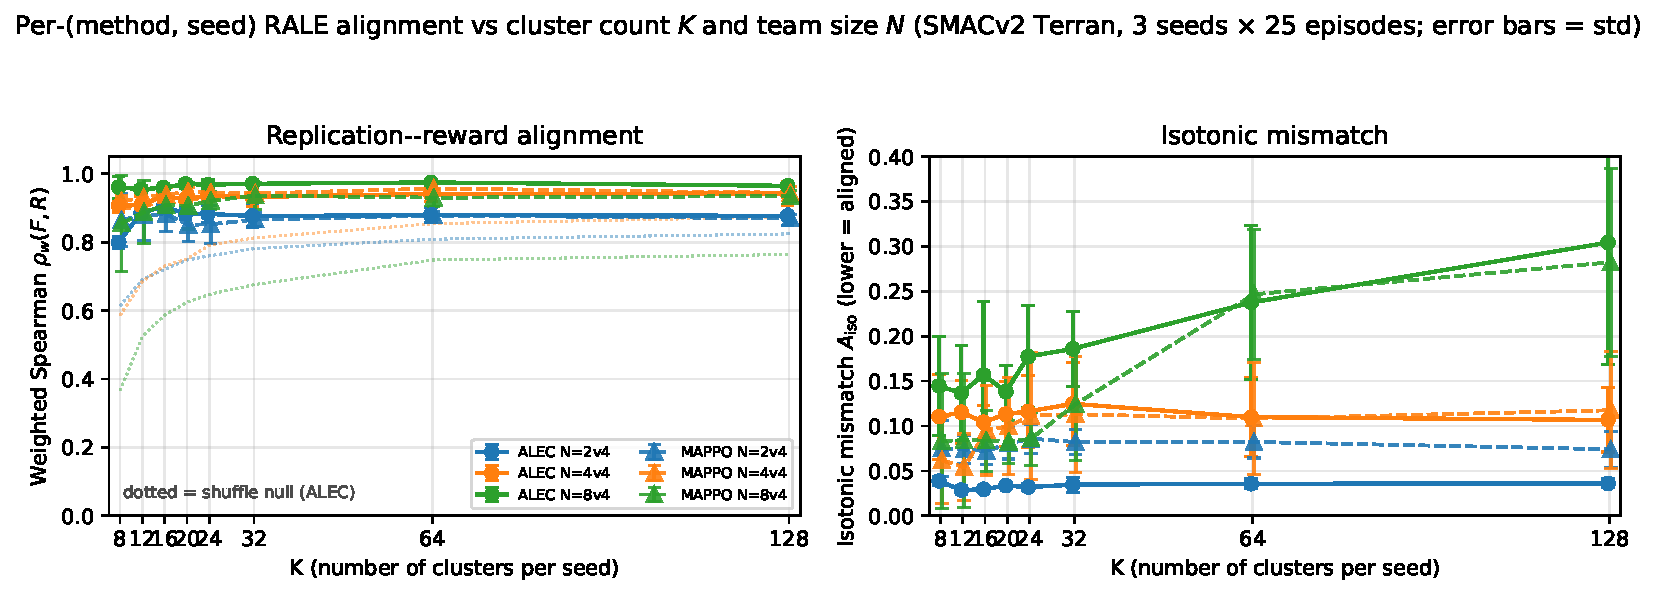
\includegraphics[width=0.99\linewidth]{figures/rale_alignment_K_N.pdf}
\caption{Per-(method, seed) RALE alignment as a function of cluster count
$K$ for SMACv2 Terran with team sizes $N\in\{2,4,8\}$ ($3$ seeds $\times$
$25$ deterministic episodes; error bars are sample standard deviation
across seeds). \textbf{Left:} weighted Spearman $\rho_w(F,R)$ (higher is
better). ALEC (circles, solid) and MAPPO (triangles, dashed) achieve
comparable raw $\rho_w$ across $(N,K)$, both well above the
$Y$-shuffle null floor (dotted, per $N$, ALEC), but ALEC's null floor is
systematically higher because its transition operator $Q$ is more diagonal.
The shuffle-corrected $\Delta\rho_w\equiv\rho_w - \rho_w^{\mathrm{shuf}}$
(Table~\ref{tab:rale-smacv2}) favours MAPPO at $7/9$ cells.
\textbf{Right:} isotonic mismatch $A_{\mathrm{iso}}$ (lower is better
aligned). ALEC has lower mismatch only at $N\!=\!2$; at $N\!\in\!\{4,8\}$
MAPPO's tighter geometry yields a more monotone $F\!\to\!R$ map.}
\label{fig:rale-K-N}
\end{figure}
